\chapter{Setting of the registers}\label{sec:codeExplain}
\fxfatal{Eitthvað að kikja á }
To configure Teensy's ADC, DMA, PDB, the datasheet of the Kinetis K64F reference manual was used \cite{freescale_semiconductor_kinetis_2021}.
The information regarding the registers of each module can be found among other things.

%\textbf{BLS 933 \cite{freescale_semiconductor_kinetis_2021}.}
Starting with the PDB  which can be seen in \textit{Listing \textbf{BÆTA VIÐ kóða}}.
Firstly the clock for the PDB clock needs to be enabled, which is done by setting the SIM\_SCGC6\_PDB;
Which for the Teensy3.5 is 60MHz default and can be scaled down using prescaler.
Since the desire was to trigger at a high frequency the prescaler and multiplier of the prescaler were both set as 1 for the high clock speed possible.
\textbf{$$input clock = \frac{F\_BUS}{\frac{prescaler}{/multiplier}} = 60MHz$$}
Then the modulus register needs to be set, which will define the frequency of which the PDB will trigger and was calculated using the equation below.

$$modulus = \frac{input clock}{sample frequency}$$

The input clock increases a counter at the rate of its speed and the modulus sets the value of which the counter will set at zero and restart its count if the PDB is in continuous mode.
Once the modulus has been determined, several registers need to be configured in order to define the PBDs operation.
Most of which is done via PDB0\_SC register, which is the status and control register for PDB on channel 0.
Firstly to enable the PDB $ PDB\_SC\_PDBEN $ is set.
Then the trigger input source is selected as software trigger, by selecting $0xf (15)$ in $ PDB\_SC\_TRGSEL $.
To have to PDB run until it is stopped, the continuous mode needs to be enabled which is done by enabling $ PDB\_SC\_CONT $.
The PDB can trigger an interrupt to do that PDB interrupts need to be enabled, which is done by enabling
$ PDB\_SC\_PDBIE $.
There needs to be set an interrupt delay when using the PDB for the interrupt, which is done by setting a value to $PDB0\_IDLY = 1;$ and the ISR is triggered when the PDB counter reaches idly value.
Once the PDB configuration has been set, the registers need to be updated which is done by $ PDB\_SC\_LDOK$.
Then a PDB pre-trigger needs to be enabled since it is used to precondition the ADC block prior to the actual ADC conversion occurs.
%\textbf{p942}
This is done by enabling the pre-trigger by enabling the $PDB0\_CH0C1\_EN$ as well as the channel pre-trigger output $PDB0\_CH0C1\_TOS$.
This is achieved by writing $0x101$ to PDB0\_CH0C1.
%\begin{figure}[h]
%    \centering
%    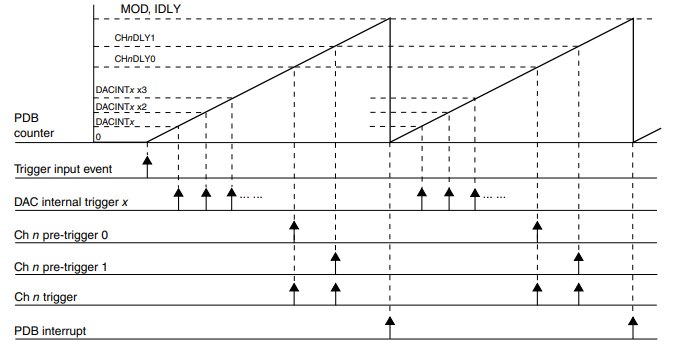
\includegraphics[width=0.70\textwidth]{graphics/PDBtrigger.png}
%    \caption{PDB ADC triggers and DAC interval triggers use case \textbf{KANSKI sleppa nennei ekki að tala um}\cite{freescale_semiconductor_kinetis_2021}}
%    \label{fig:PDBTrigger}
%\end{figure}
Then the ADC can be configured first, the conversion mode needs to be determined.
The built-in ADC is up to 16bit and can be configured to run at 8-, 10-, 12- and 16-bit resolution modes, which is done through $ADC\_CFG1\_MODE$.
Two different reference voltages can be set, for the configuration of the circuit analog ground pin is used instead of an internal ground.
To achieve this $ADC0\_SC2$ needs to be set to 0.
Since the ADC is supposed to PDB trigger, that needs to be enabled.
$ADC\_SC2\_ADTRG$ sets the ADC to be hardware triggered, which in this case is set to be the PDB.
DMA transfer needs to be enabled here so that the conversion values of the ADC can go straight to memory, which is done by enabling  $ADC\_SC2\_DMAEN$.
All that is left is to select the analog pin, which is done by writing the pin hex value to $ADC0\_SC1A$ which in this case was "A9" or 0x04, see page 120 in \cite{freescale_semiconductor_kinetis_2021}.
The results of each conversion are then stored in $ADC0\_RA$ data result register.

Lastly the DMA is configured, to help with the process "DMAChannel.h" was used, which is a Teensy library.
Multiple registers need to be configured and set.
For instance where the data is coming from, where it is supposed to be delivered and when to go into the interrupt service routine (ISR) to name a few.
To initiate a DMA channel DMA.begin() is called.
Then the trigger for when the DMA transfer is supposed to occur needs to be set, which is done by setting the service request trigger as when an ADC conversion occurs.
This is done by configuring the $dma.triggerAtHardwareEvent$ as seen here $dma.triggerAtHardwareEvent(DMAMUX\_SOURCE\_ADC0)$.
Which sets in motion the DMA transfer.
Defining the source address $dma.TCD->SADDR$ needs to be set in this case, the location of the results of the ADC conversion, $ADC0\_RA$.
If the source address changes between each DMA transfer, there needs to be an offset put on the address which is done via $dma.TCD->SOFF$. 
Which in this case is 0 bytes, since $ADC0\_RA$ is just overwritten for each ADC conversion and its address does not change.
If the source address changes between each ISR call then adjustments can be made through $dma.TCD->SLAST$, which also does not change and is still the address of $ADC0\_RA$.
The data that is incoming and supposed to be transmitted needs to be set, which in this project is 2 bytes since the ADC will be configured in an above 8bit resolution.
This is done by $dma.TCD->ATTR = DMA\_TCD\_ATTR\_SSIZE(1) | DMA\_TCD\_ATTR\_DSIZE(1);$ which defines 16bit data transfers.
Which firstly defines the size of the incoming data as well as defining the destination data transfer size.
The number of bytes to transfer for each service request $DMAMUX\_SOURCE\_ADC0$ which is done with  $dma.TCD->NBYTES_MLNO = 2;$, this is considered a minor loop .
Then the destination source needs to be set like before, $dma.TCD->DADDR = dmaBuf;$ defines the destination address to a DMA buffer called dmaBuf which is defined in the main program.
This time there needs to be an offset is set to the address since the DMA is writing to a buffer to store the value instead of just overwriting the value like it was for the source.
This is done by setting the destination offset as the size of the ADC conversion value, or 2 bytes $dma.TCD->DOFF = 2;$.
To keep track of how many values have been set through DMA, the  $dma.TCD->CITER\_ELINKNO $ counter is set as the size of the buffer that the DMA values are being transferred to.
This value is decremented each time a value has been transferred via service request and transfer.
Since in the main program dmaBuf is 2 arrays of a size of 128 indexes this is set to 128 \textbf{Staðfesta!}.
When the count reaches 0, meaning the DMA buffer is full.
The counter needs to be reset back to its original value, this is done by setting $dma.TCD->BITER\_ELINKNO$ as the same value as the counter was set as.
The destination of the last address adjustment for the next transfer needs to be set, which is done by $dma.TCD->DLASTSGA = -sizeof(dmaBuf);$
When both DMA buffers are full, DMA resets, so it can rewrite to the first buffer.
To define when the ISR occurs, the $dma.TCD->CSR $ is set.
Since the BITER register was also set the reference manual states to use $DMA\_TCD\_CSR\_INTMAJOR$, however this resulted in only half the data being transmitted so $DMA\_TCD\_CSR\_INTMINOR$ was also set.
This sets DMA to trigger twice once when the first DMA buffer is full as well as when the second buffer is full.

Finally the DMA channel is enabled by $dma.enable();$.
The DMA ISR is used to transfer the data from the dmaBuf to fifoBuf in order to transfer it to the SD card later on. 